% Template for WHISPERS-2009 paper; to be used with:
%          stywhispers.sty  - WHISPERS LaTeX style file, and
%          IEEEbib.bst - IEEE bibliography style file.
% --------------------------------------------------------------------------
% Template for IGARSS-2020 paper; to be used with:
%          spconf.sty  - LaTeX style file, and
%          IEEEbib.bst - IEEE bibliography style file.
% --------------------------------------------------------------------------
\documentclass{article}
\usepackage{spconf,amsmath,epsfig, amsfonts, amssymb, xcolor, hyperref, caption, subcaption, graphicx, xcolor}
\urlstyle{same}
\usepackage[linesnumbered,ruled,vlined]{algorithm2e}
\usepackage[utf8]{inputenc}
\usepackage[english]{babel}
\newtheorem{definition}{Definition}
\usepackage{algorithmic}
\newcommand{\argmin}{\operatornamewithlimits{argmin}}% Example definitions.
\DeclareMathOperator*{\argmax}{argmax} % thin space, limits underneath in displays% --------------------
\def\x{{\mathbf x}}
\def\R{\mathbb{R}}
\def\L{{\cal L}}


% Example definitions. 


% --------------------
\def\x{{\mathbf x}}
\def\hx{{\hat x}}
\def\L{{\cal L}}
\def\R{{\mathbb R}}
\def\E{{\mathbb E}}
\newcommand{\Dt}{\mathcal{D}_{t}}
\newcommand{\JMM}[1]{{\textcolor{blue}{[#1]}}}


% Title.
% ------
\title{Deep Diffusion Processes for Active Learning of Hyperspectral Images}
%
% Single address.
% ---------------
\name{Duc Nguyen$^{1}$, Abiy Tasissa$^{2}$, James M. Murphy$^{2}$
\thanks{D.N. and A.T. are joint first authors.  This research is partially supported by the US National Science Foundation grants NSF-DMS 1912737, NSF-DMS 1924513, and NSF-CCF 1934553.}}
\address{$^{1}$Department of Mathematics, University of Maryland, College Park, USA\\ 
$^{2}$Department of Mathematics, Tufts University, USA
	}


\begin{document}

\maketitle

\begin{abstract} A method for active learning of hyperspectral images (HSI) is proposed, which combines deep learning with diffusion processes on graphs.  A deep variational autoencoder extracts smoothed, denoised features from a high-dimensional HSI, which are then used to make labeling queries based on graph diffusion processes.  The proposed method combines the robust representations of deep learning with the mathematical tractability of diffusion geometry, and leads to strong performance on real HSI.  

\end{abstract}

\begin{keywords}hyperspectral images, variational autoencoders, deep clustering, active learning, semisupervised learning, diffusion geometry\end{keywords}

\section{Introduction}
\label{sec:Introduction}
 
 Machine learning has provided revolutionary new tools for remote sensing, but state-of-the-art methods often require huge labeled training sets.  In particular, supervised deep learning methods can achieve near-perfect labeling accuracy on high-dimensional hyperspectral images (HSI), provided large libraries of labeled pixels are available \cite{Zhu2017_Deep}.  This hinders the practicality of these methods, as in many settings, data is collected at a pace that far exceeds human ability to generate corresponding labeled training data.
 
 In order to account for this, methods that require only a very small number of labels are needed.  The \emph{active learning} regime is particularly attractive for HSI labeling problems.  In active learning, an algorithm is provided with an unlabeled dataset, and the algorithm iteratively queries points for labels.  By choosing query points intelligently, the active learning algorithm can yield the classification performance of a much larger training set chosen uniformly at random.  
 
 We propose an active learning method for HSI based on deep feature extraction and random walks on graphs.  First, an unsupervised variational autoencoder is used to nonlinearly denoise and compress the high-dimensional HSI.  Then, the resulting features are considered as vertices of a graph, and a Markov diffusion process on the graph is used to determine label queries and label all data points.  The proposed method combines the efficient feature learning of deep autoencoders with the mathematical interpretability of graph diffusion processes, and leads to strong empirical performance on real HSI.  

%%%
%%%

\section{Variational Autoencoders }

We now describe VAEs following the exposition in \cite{yang2018geodesic}. Let $x \in \R^N $ and consider a latent variable model $p_{\theta}(x) = \int p(x|z;\theta)p(z)\,dz$. The variable $z\in \R^{D}$, $D\ll N$, is a latent variable and provides a low-dimensional parametrization of the data $x$. The goal of VAE is to maximize the probability of  data samples generated as $p(x)$. In the inference part of VAE, the training procedure maps a data point $x$  to its latent representation $z$ such that the $z$ adheres to the distribution $p(z)$. 

Since the posterior distribution $p(z|x)$ and $p(z)$ are unknown, VAE makes the assumption that $p(z|x) = q(z|x,\phi)$ where $\phi$ are parameters to be learned from the network. To enforce that the variational distribution $q(z|x,\phi)$ agrees with $p(z)$, the optimization $\min_{\phi}\,\, KL(q(z|x,\phi),p(z))$ is considered, where KL is the Kullback-Leibler divergence.  With this, $q(z|x)$ can be interpreted as the encoder part of VAE providing us a latent representation $z$ given a sample $x$. 

The generative part of VAE considers the reconstruction of a data sample given the latent representation $z$. In particular, the goal of the training procedure is to map a latent variable $z$ to a data sample $\hat{x}$ such that $\hat{x}$ is similar to the true data sample $x$. This naturally motivates the maximization of $p(x|z,\theta)$ with $\theta$ denoting the network parameters. Formally, we consider the optimization program $\max_{\theta}\, \E_{z \sim q(z|x,\phi)} \log p(x|z;\theta)$.  With this, $p(x|z)$ can be interpreted as the decoder part of VAE. The inference and generative parts of VAE i.e the encoder and decoder model can be jointly trained by maximizing the loss function $$\mathcal{L}(x,z;\theta,\phi)
=  \displaystyle\mathop{\E}_{z\sim q(z|x,\phi)} \log p(x|z;\theta)- KL(q(z|x,\phi),p(z))$$ In summary, the optimal network parameters $\theta^{*}$ and $\phi^{*}$ are obtained as $(\theta^{*},\phi^{*})=\argmax_{\theta,\phi} \mathcal{L}(x,z;\theta,\phi)$, optimized using stochastic gradient descent.  Intuitively, the encoding of $x\in\mathbb{R}^{N}$ by $z\in\mathbb{R}^{D}$ for $D\ll N$ is an efficient low-dimensional representation of the data which ideally captures the underlying statistics and geometry of the data.  In our proposed methodology, the latent space representation resulting from a trained VAE is used as input to a clustering algorithm which suggests candidate points to query for labels.

\subsection{Learning by Active Nonlinear Diffusion}
In this paper, we use an active learning algorithm for high dimensional data based on diffusion geometry \cite{Murphy2019_Unsupervised, Maggioni2019_LUND, Murphy2020_Spectral}. The algorithm, learning by active nonlinear diffusion (LAND) \cite{Maggioni2019_LAND}, is a semisupervised algorithm that takes into account the geometry of the data to identify the most important points to be query for labels. A key advantage of LAND is that it provides rigorous theoretical performance guarantees and handles general clusters that could be nonlinear, live in a high ambient dimension, and may be corrupted by noise and outliers \cite{Maggioni2019_LAND}.

Consider an HSI $X=\{x_{i}\}_{i=1}^{n}\subset\mathbb{R}^{m}$, where each pixel is represented as a point in $\R^{m}$ where $m$ is the number of spectral bands. Let $W$ to be the $n\times n$ weight matrix defined as $W_{ij}=\exp(-\|x_{i}-x_{j}\|_{2}^{2}/\sigma^{2}), x_{j}\in NN_{k}(x_{i})$ and $W(x_{i},x_{j})=0$ otherwise, where $NN_{k}(x_{i})$ is the set of $k$-nearest neighbors of $x_{i}$ in $X$ with respect to Euclidean distance and $\sigma$ is a scale parameter. Given the weight matrix, the degree of $x$ is $\deg(x_{i}):=\sum_{x_{j}\in X}W_{ij}$. A random walk on $X$ can be defined using the $n\times n$ transition matrix $P_{ij}={W_{ij}}\big/{\deg(x_{i})}.$  
By construction, $P$ has a spectral decomposition $\{(\lambda_{i},\Psi_{i})\}_{ni=1}^{n}$, and we define the \emph{diffusion distance at time $t$} between $x_{i},x_{j}\in X$ as $D_{t}(x_{i},x_{j})=\sqrt{\sum\nolimits_{\ell=1}^{n}\lambda_{\ell}^{2t}(\Psi_{\ell}(x_{i})-\Psi_{\ell}(x_{j}))^{2}}$.  The parameter $t$ in diffusion distance depends on a parameter $t$ informs how long the diffusion process runs.  In this paper, we set $t$ to be 30; diffusion learning is relatively robust to choice of $t$ \cite{Murphy2019_Unsupervised}. 

An important part of the LAND algorithm is to determine the data points which one should query for labels. This is achieved using a kernel density estimator and diffusion geometry.  Consider the density estimator $p(x)=\sum_{y\in NN_{k}(x)}\exp(-\|x-y\|_{2}^{2}/\sigma_{0}^{2})$
with $\sigma_0$ denoting a scale parameter. Let 
\begin{align}\label{eqn:rho}
\rho_{t}(x) &=
\begin{cases}
\displaystyle\min_{p(y)\ge p(x), x\neq y} D_{t}(x,y), &x\neq \displaystyle\argmax_{z}p(z) \\
\displaystyle\max_{y\in X} D_{t}(x,y), & x=\displaystyle\argmax_{z}p(z)
\end{cases}
\end{align} be the ($t$-dependent) diffusion distance between a point and its nearest diffusion neighbor of higher density if $x$ is not the maximizer of $p(x)$, and the maximum diffusion distance to another point if $x$ is the maximizer of $p(x)$.  The modes of the data are determined as the maximizers of $\Dt(x)=p(x)\rho_{t}(x)$.  A large $\Dt$ value indicates a high-density point that is $D_{t}$-far from other high density points. In LAND, the modes of $X$ are characterized as maximizers of $\Dt$. Diffusion distances and density can also employed to label all other points relative to these modes. We refer the interested reader to 
\cite{Maggioni2019_LAND}. 


\subsection{Related Work}
%We propose an active learning algorithm which has two main stages. The first stage is feature extraction of an unlabeled high-dimensional dataset using a variational autoencoder. The second stage employs an active learning diffusion based clustering algorithm to infer the true labels. In what follows, we describe these two stages in detail. 
Extracting essential features of data is an important part of both supervised and unsupervised machine learning problems. For example, the unsupervised technique of Gaussian mixture models (GMM) assumes that the data under consideration is an i.i.d. sample from a mixture of Gaussians, and the parameters of the GMM are estimated by expectation maximization \cite{Murphy2012_Machine}. In recent years, deep generative methods, such as \emph{generative adversarial network (GANs)} and \emph{variational autoencoder networks (VAEs)}, have been used as feature extraction tools and successfully applied to many machine learning tasks \cite{ehsan2017infinite,makhzani2015adversarial}. In the context of the clustering problem, a set of methods, known as deep clustering, propose learning features of the data and clustering simultaneously, showing strong empirical results \cite{tian2014learning,song2013auto,xie2016unsupervised,jiang2017variational}. 
In the context of HSI images, several works have employed different deep learning architectures to extract essential features for downstream tasks such as classification
\cite{chen2014deep,chen2016deep,li2017spectral,he2017multi,paoletti2019deep,zhang20191d}. 

Active learning is a learning paradigm where the user has the ability to select the training data\cite{cohn1995active,mackay1992information}.  Consider unlabeled data $\{\x_1,\x_2,...,\x_n\}$ in $\mathbb{R}^{m}$ with corresponding true labels $\{y_1,y_2,...,y_n\}$. In active learning, the user can obtain labels for at most $B<n$ of the data points. Hereafter, we refer to $B$ as the fixed budget the user has access to. The underlying idea is that a few informative training samples could be sufficient for training an algorithm and obtaining accurate results. Given this, active learning methods differ in the way these informative samples are chosen. This learning framework has been used in remote sensing for hyperspectral image classification \cite{liu2016active,wang2017novel,murphy2018iterative,tuia2009active}.  This list is by no means comprehensive and we refer the interested reader to the survey in \cite{tuia2011survey}. 
The main idea in this paper is that the active learning process depends on the representation and geometry of the data. For the former, we use deep neural networks to extract low
dimensional features. To sample training data, restricted to the budget $B$, we employ a diffusion process based approach that is provably robust to geometry of the data. 
 The closest work to ours is  \cite{pourkamali2019effectiveness} where the authors combine active learning with variational autoencoders. Therein, K-means clustering is first used to partition the space and then labels are acquired using uniform random sampling in each partition. Given the labels, a classifier is then trained in the latent space for the prediction task. The underlying assumption is that the K-means partitions represent the structure of the latent space, and empirical results in \cite{pourkamali2019effectiveness} show the superiority of this approach to doing active learning via K-means partitions in the original space. Since the performance of the active learning algorithm hinges on how well the geometry of the latent space is represented, the choice of the clustering method is crucial. One of the highlights of the proposed method is that the clustering algorithm LAND is theoretically grounded and handles a more broad class of cluster geometries than K-means does.

\section{Proposed Algorithm}
\label{sec:ProposedAlgorithm}
We propose an active learning algorithm, VAE-LAND (see Algorithm \ref{alg:VALAND}), which has two main stages. The first stage is feature extraction of an unlabeled high-dimensional dataset using a variational autoencoder. The second stage employs the LAND active learning diffusion based clustering algorithm to infer the true labels.  The second part of the algorithm concerns deploying clustering algorithms on the latent representation of the data. Since our algorithm is in the active learning framework, we first acquire labels for small subset of the latent data. Different active learning algorithms differ in the ways in which one determines the subset of the data to query for labels.  The proposed algorithm combines the power of variational autoencoders to extract features and uses diffusion geometry on graphs to find impactful labels to query, which then propagate to other points. 

%To summarize, our proposed algorithm has two main steps.  We first use an unsupervised VAE to perform a low-dimensional embedding on the data and then second cluster the latent representation of the data using LAND. 

\RestyleAlgo{boxruled}
\begin{algorithm}[!htb]
	\caption{\label{alg:VALAND}Variational Autoencoder Learning by Active Nonlinear Diffusion (VALAND)}
	\flushleft
	\flushleft
	\textbf{Input:} $\{x_{i}\}_{i=1}^{n}$ (Unlabeled Data); $\{(\lambda_{\ell},\psi_{\ell})\}_{\ell=1}^{M}$ (Spectral Decomposition of $P$); $\{p(x_{i})\}_{i=1}^{n}$ (Kernel Density Estimate);  $\{\rho_{t}(x_{i})\}_{i=1}^{n}$ (\ref{eqn:rho}); $t$ (Time Parameter); $B$ (Budget); $\mathcal{O}$ (Labeling Oracle)
	
	\vspace{5pt}
	
	\textbf{Output:} $Y$ (Labels)
	
		\vspace{5pt}


	\begin{algorithmic}[1]
	\STATE Run VAE on unlabeled data to obtain  the latent representation $X = \{\hx_{i}\}_{i=1}^{n}$.  
	\STATE Compute $\Dt(\hx_{i})=p(\hx_{i})\rho_{t}(\hx_{i})$.  
	\STATE Sort the data in decreasing $\Dt$ value to\ 
	acquire the ordering $\{\hx_{m_{i}}\}_{i=1}^{n}$.\FOR{$i=1:B$}
	\STATE Query $\mathcal{O}$ for the label $L(\hx_{m_{i}})$ of $\hx_{m_{i}}$.
	\STATE Set $Y(\hx_{m_{i}})=L(\hx_{m_{i}})$.
	\ENDFOR
	\STATE Sort $X$ according to $p(\hx)$ in decreasing order as $\{\hx_{\ell_{i}}\}_{i=1}^{n}$.  
	\FOR{$i=1:n$}
	\IF{$Y(\hx_{\ell_{i}})=0$}
	\STATE $Y(\hx_{\ell_{i}})=Y(z_{i}), \, z_{i}=\displaystyle\argmin_{z}\{D_{t}(z,\hx_{\ell_{i}})$\ $| \ $ $p(z)>p(\hx_{\ell_{i}}) \text{ and } Y(z)>0\}$.
	\ENDIF
	\ENDFOR
	\end{algorithmic}
\end{algorithm}


\section{Experimental Results}
\label{sec:Experiments}
We demonstrate the accuracy of the proposed algorithm by running numerical experiments. The training of the VAE is done using Tensorflow in Python. For doing the clustering via LAND, we use the publicly available MATLAB code 
at  \url{https://jmurphy.math.tufts.edu/Code/}. Our code can be found at \url{https://github.com/abiy-tasissa/VAE-LAND}. Our test HSI dataset is the Salinas A hyperspectral dataset. The Salinas scene was captured over Salinas Valley, California. The image has a spatial resolution of 3.7-meter pixels and contains 224 spectral bands. The ground truth consists of 16 classes. We consider the Salinas A dataset, which is a subset of the Salinas dataset, and contains 6 classes. The Salinas A dataset and the ground truth data are publicly available (\url{http://www.ehu.eus/ccwintco/index.php/Hyperspectral_Remote_Sensing_Scenes#Salinas-A_scene}). Figure \ref{fig:SalinasA} shows a visual of the high dimensional data and the ground truth labels. The performance of the algorithm is assessed using overall accuracy, defined as the ratio of correctly estimated labels to total number of labels. 

\begin{figure}[htb]
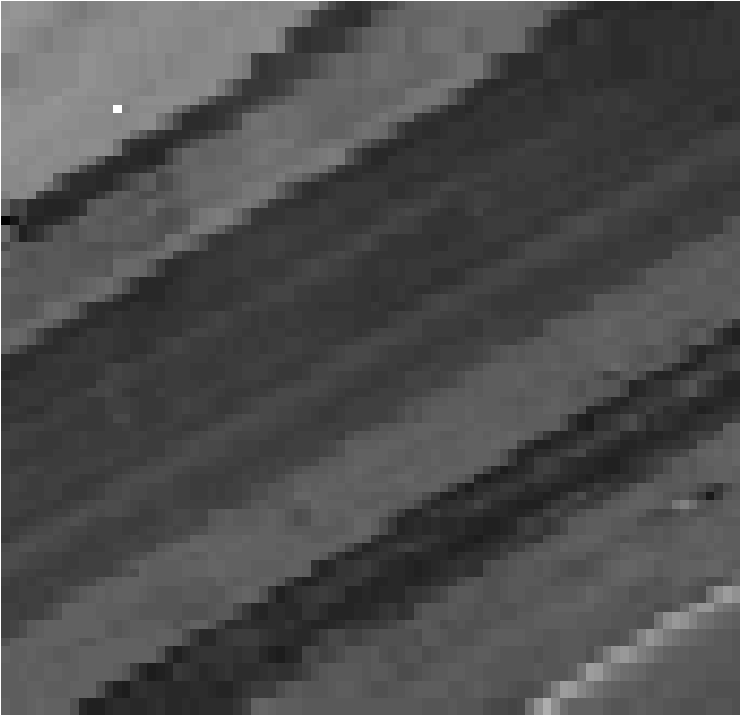
\includegraphics[width=.23\textwidth,clip]{Images/SalinasA_BandSum-crop.pdf}
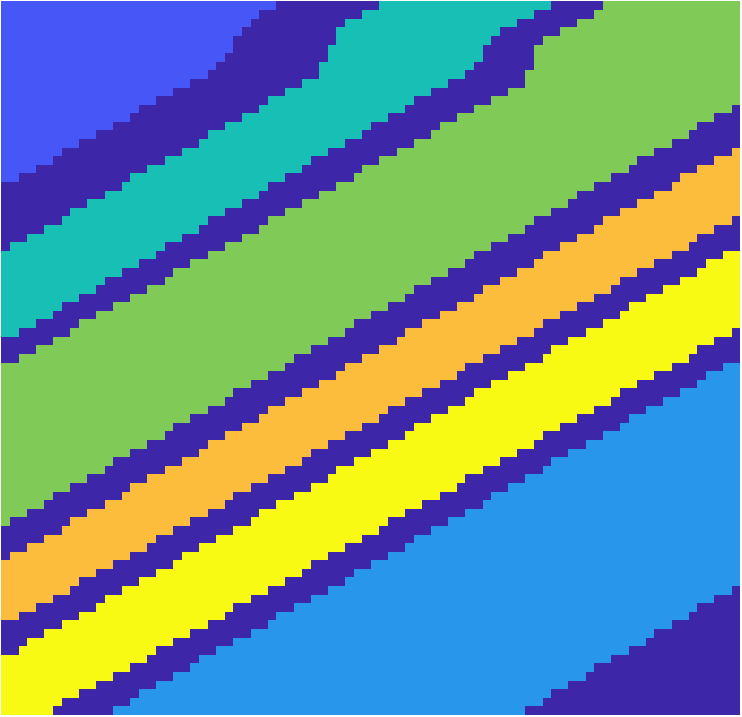
\includegraphics[width=.23\textwidth,clip]{Images/SalinasA_GT-crop.pdf}
\caption{\small{The $86\times 83$ Salinas A HSI data consists of 6 classes.  Left: the sum of all spectral bands.  Right: the ground truth.}}
\label{fig:SalinasA}
\end{figure}

\begin{figure}[htb]
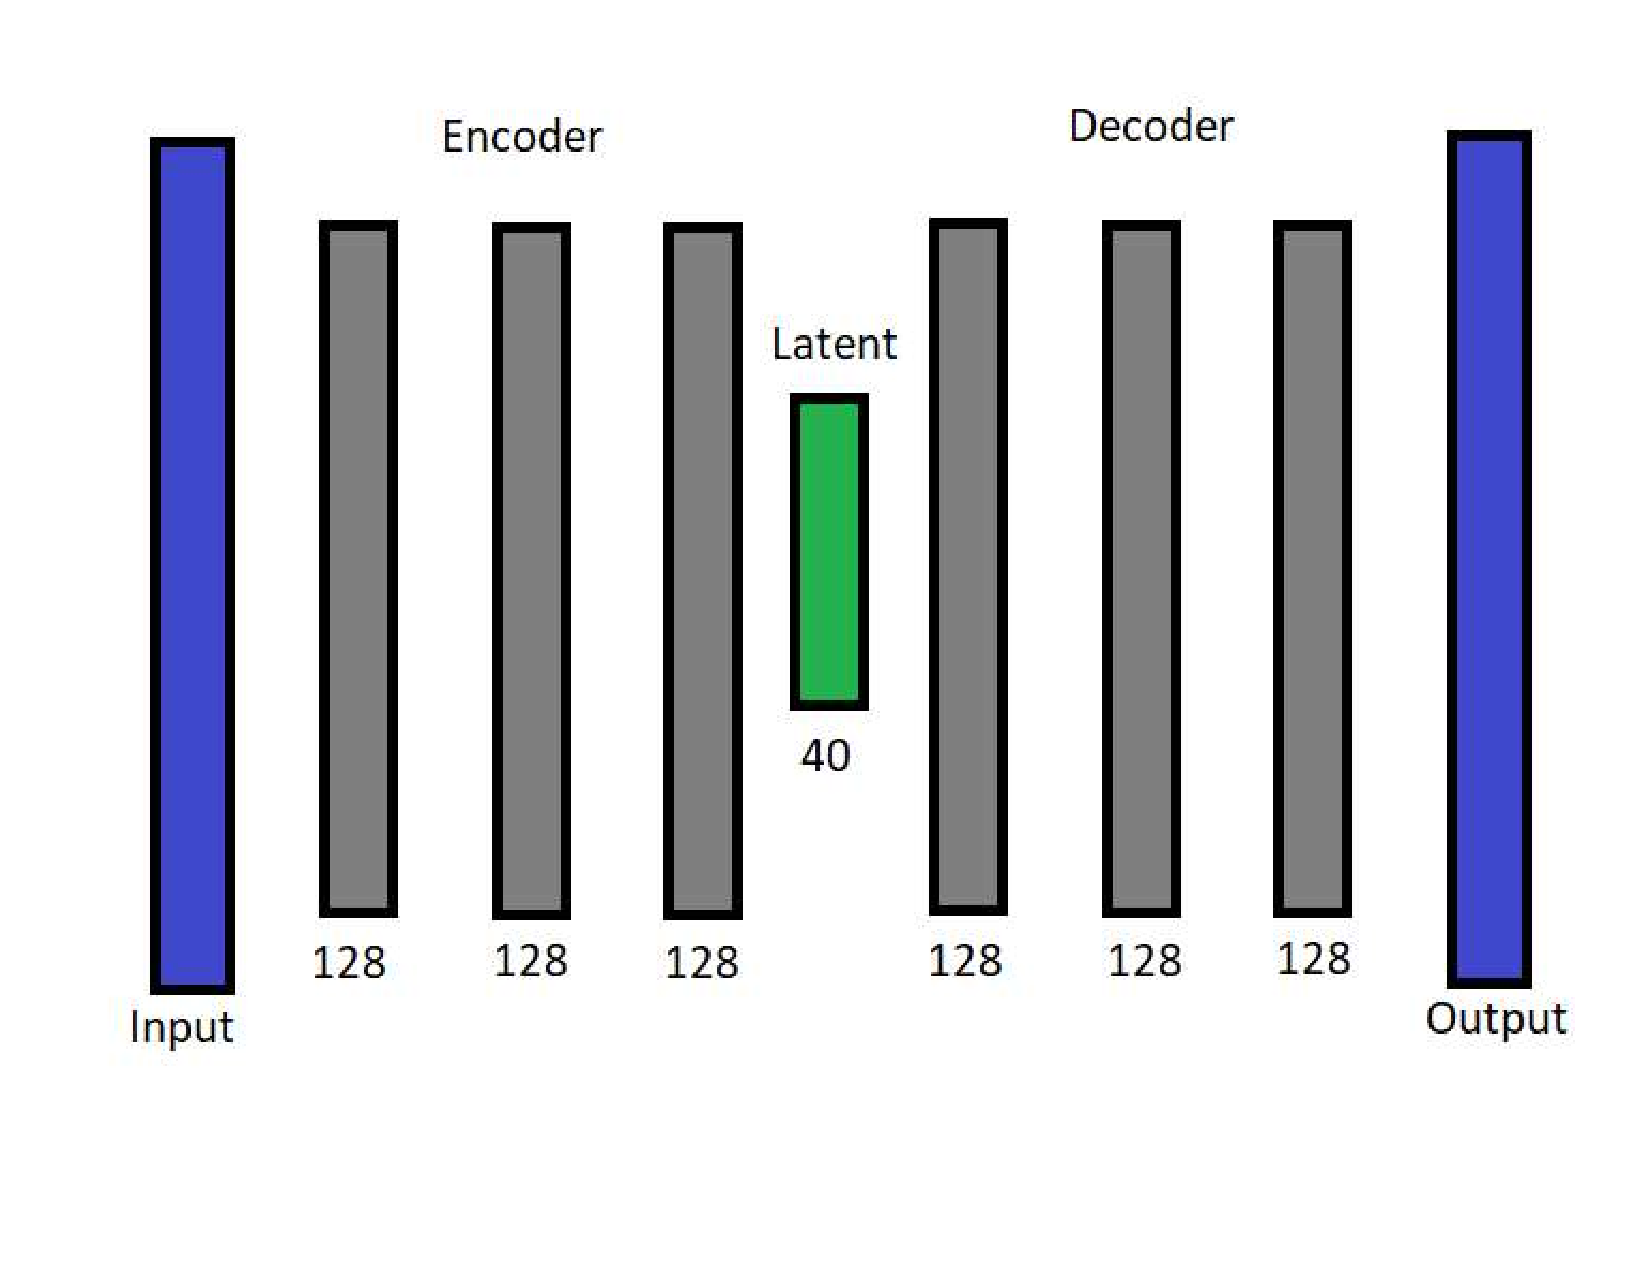
\includegraphics[clip,width=.45\textwidth,trim=1cm 3.5cm 1cm 1cm]{Images/VAE_Schematics.pdf}
\caption{\small{A schematics of the VAE archiecture. Input is cascaded through an encoder, three dense layers of size 128. The extraccted latent feature is fed to the decoder,three dense
layers of size 128, to obtain the output. Note, unlike the standard autoencoder, the extraction of the latent feature is not deterministic.   }}
\label{fig:SalinasA}
\end{figure}
The Salinas A HSI dataset of size $83 \times 86\times 224$ is represented as a point cloud of size $7138\times 224$. We use the unlabeled data to learn a latent space representation of Salinas A in $\R^{40}$ dimensions. The encoder network consists of three dense layers with $128$ units. The activation function is the rectified linear unit (RELU). The loss function is optimized using the Adam algorithm with learning rate set to $0.0001$. After training the VAE, we input the latent space representation of the Salinas A dataset to the LAND algorithm for the task of inferring the ground truth labels of the HSI data. We compare our result to the ``plain" LAND algorithm that simply clusters the Salinas A dataset in its original representation. Since LAND is an active learning framework, we consider varying number of labeled data points ranging from $10$ to $2000$. In addition, we want to compare the active learning methods to query the samples with randomly selected training data. Figure \ref{fig:SalinasA} compares the performance of LAND and performance of VAE-LAND. First, for both VAE-LAND and standard LAND, LAND queries lead to significantly better accuracy than random queries. The proposed algorithm, VAE-LAND, attains an accuracy of 96.97\% with just 10 labeled points. This is a $12.5\%$ improvement to the accuracy of the plain LAND algorithm for the same number of labeled points. The standard LAND algorithm requires $400$ labeled points to reach accuracy of $90\%$ while for the same number of labeled points, VAE-LAND has an accuracy of $98.35\%$. 

\noindent \textbf{Complexity and run time}: The complexity of LAND is $O(C_{NNN}+nK_{NN}+n\log(n))$ where $C_{NN}$ is the cost of computing all $K_{NN}$ nearest neighbours \cite{Maggioni2019_LAND}. 
The computational cost of VAE is difficult to estimate as it depends on several factors (e.g architecture, activation function, choice of SGD algorithm). In our numerical experiments, the cost of VAE is the dominating cost. Since LAND runs on low dimensional features extracted from VAE, it is efficient. 

\begin{figure}
   % \centering
    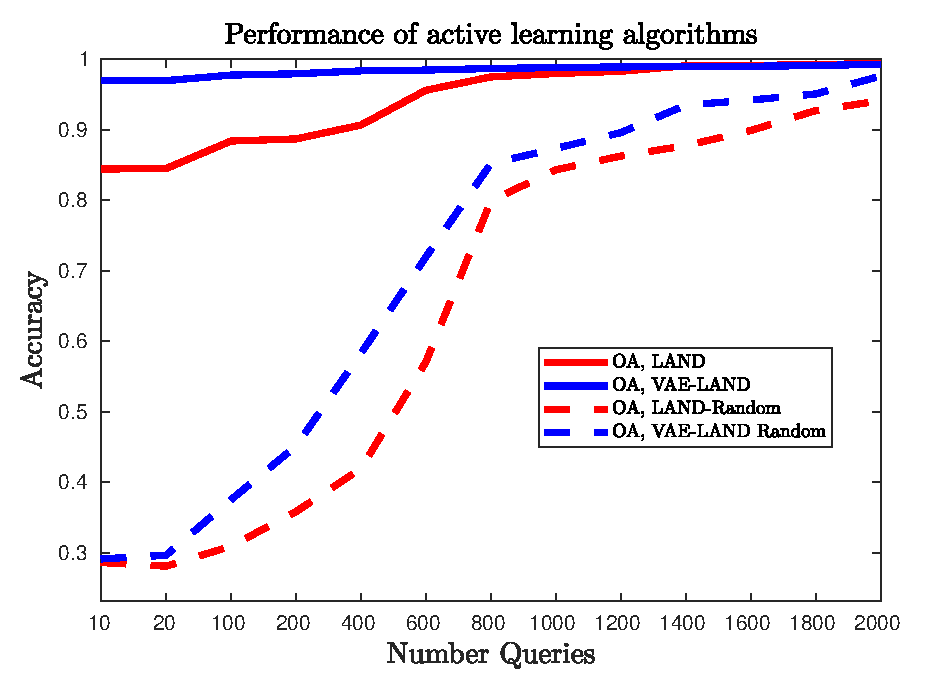
\includegraphics[width=.45\textwidth]{Images/salinasa_results_improved.eps}
    \caption{For the Salinas A dataset, the performance of variational autoencoder LAND learning achieves a higher accuracy than the standard LAND algorithm. With just $10$ points, the overall accuracy of VAE-LAND is 96.97\%, a 12.5\% improvement to the competitive LAND algorithm. Both VAE-LAND and LAND obtain significantly better results than using randomly selected training instances. }
    \label{fig:my_label}
\end{figure}


\section{Conclusions and Future Directions}
\label{sec:Conclusions}
The proposed active learning algorithm, VAE-LAND, improves over the standard LAND and gives accurate results even when the number of queries are limited. The method uses VAE to generate good features, and uses the diffusion geometry based LAND algorithm to determine query points. The LAND algorithm then uses this queried labels to predict the labels of the unlabeled data samples. In future work, we would like to explore the kind of data models for which the algorithm has theoretical performance guarantees.   


\bibliographystyle{IEEEbib}
\bibliography{IGARSS2021_ref}

\end{document}
